\documentclass[a4paper,10pt]{article}
\usepackage{graphicx,color}
\usepackage[margin=2cm]{geometry}
\usepackage{algorithm2e}

\begin{document}

{\LARGE{\centerline{\bf Lab 1}}}

\section{Matrix Addition}

\subsection{Two dimensional matrices}

\subsection{Three dimensional matrices}

\section{Matrix Multiplication}

Matrix C is the result of multiplying matrix A and B.
In two dimensions, both A and B are square matrices of equal size, N.
In three dimensions, both A and B are cubic matrices of equl size, N.
The matrices A and B are populated with random values that range 0 - 20.
N is set to 10 and 20.

\subsection{Two Dimensional Matrices}

Each element in matric C is found using equation \ref{2Dmult}.

\begin{equation}\label{2Dmult}
c_{i,j}=\sum_{k} a_{i,k} \times b_{k,j}
\end{equation}

This is achieved using three seperate \textit{for} loops.
The first \textit{for} loop traverses the rows of C, while the second \textit{for} loop traverses the columns.
The third \textit{for} loop traverses the row and column of matrices A and B.

\subsection{Three Dimensionl Matrices}

To obtain each element in matrix C, matrix A and B are divided into two dimensional matrices, A' and B'.
For each two dimensional matrix, a single row and column is multiplied to get the corresonding element in the C matrix.
This leads to a single value which is the element in the C matrix.
This is done for all elements in the c matrix.

\begin{figure}[h]
\centering
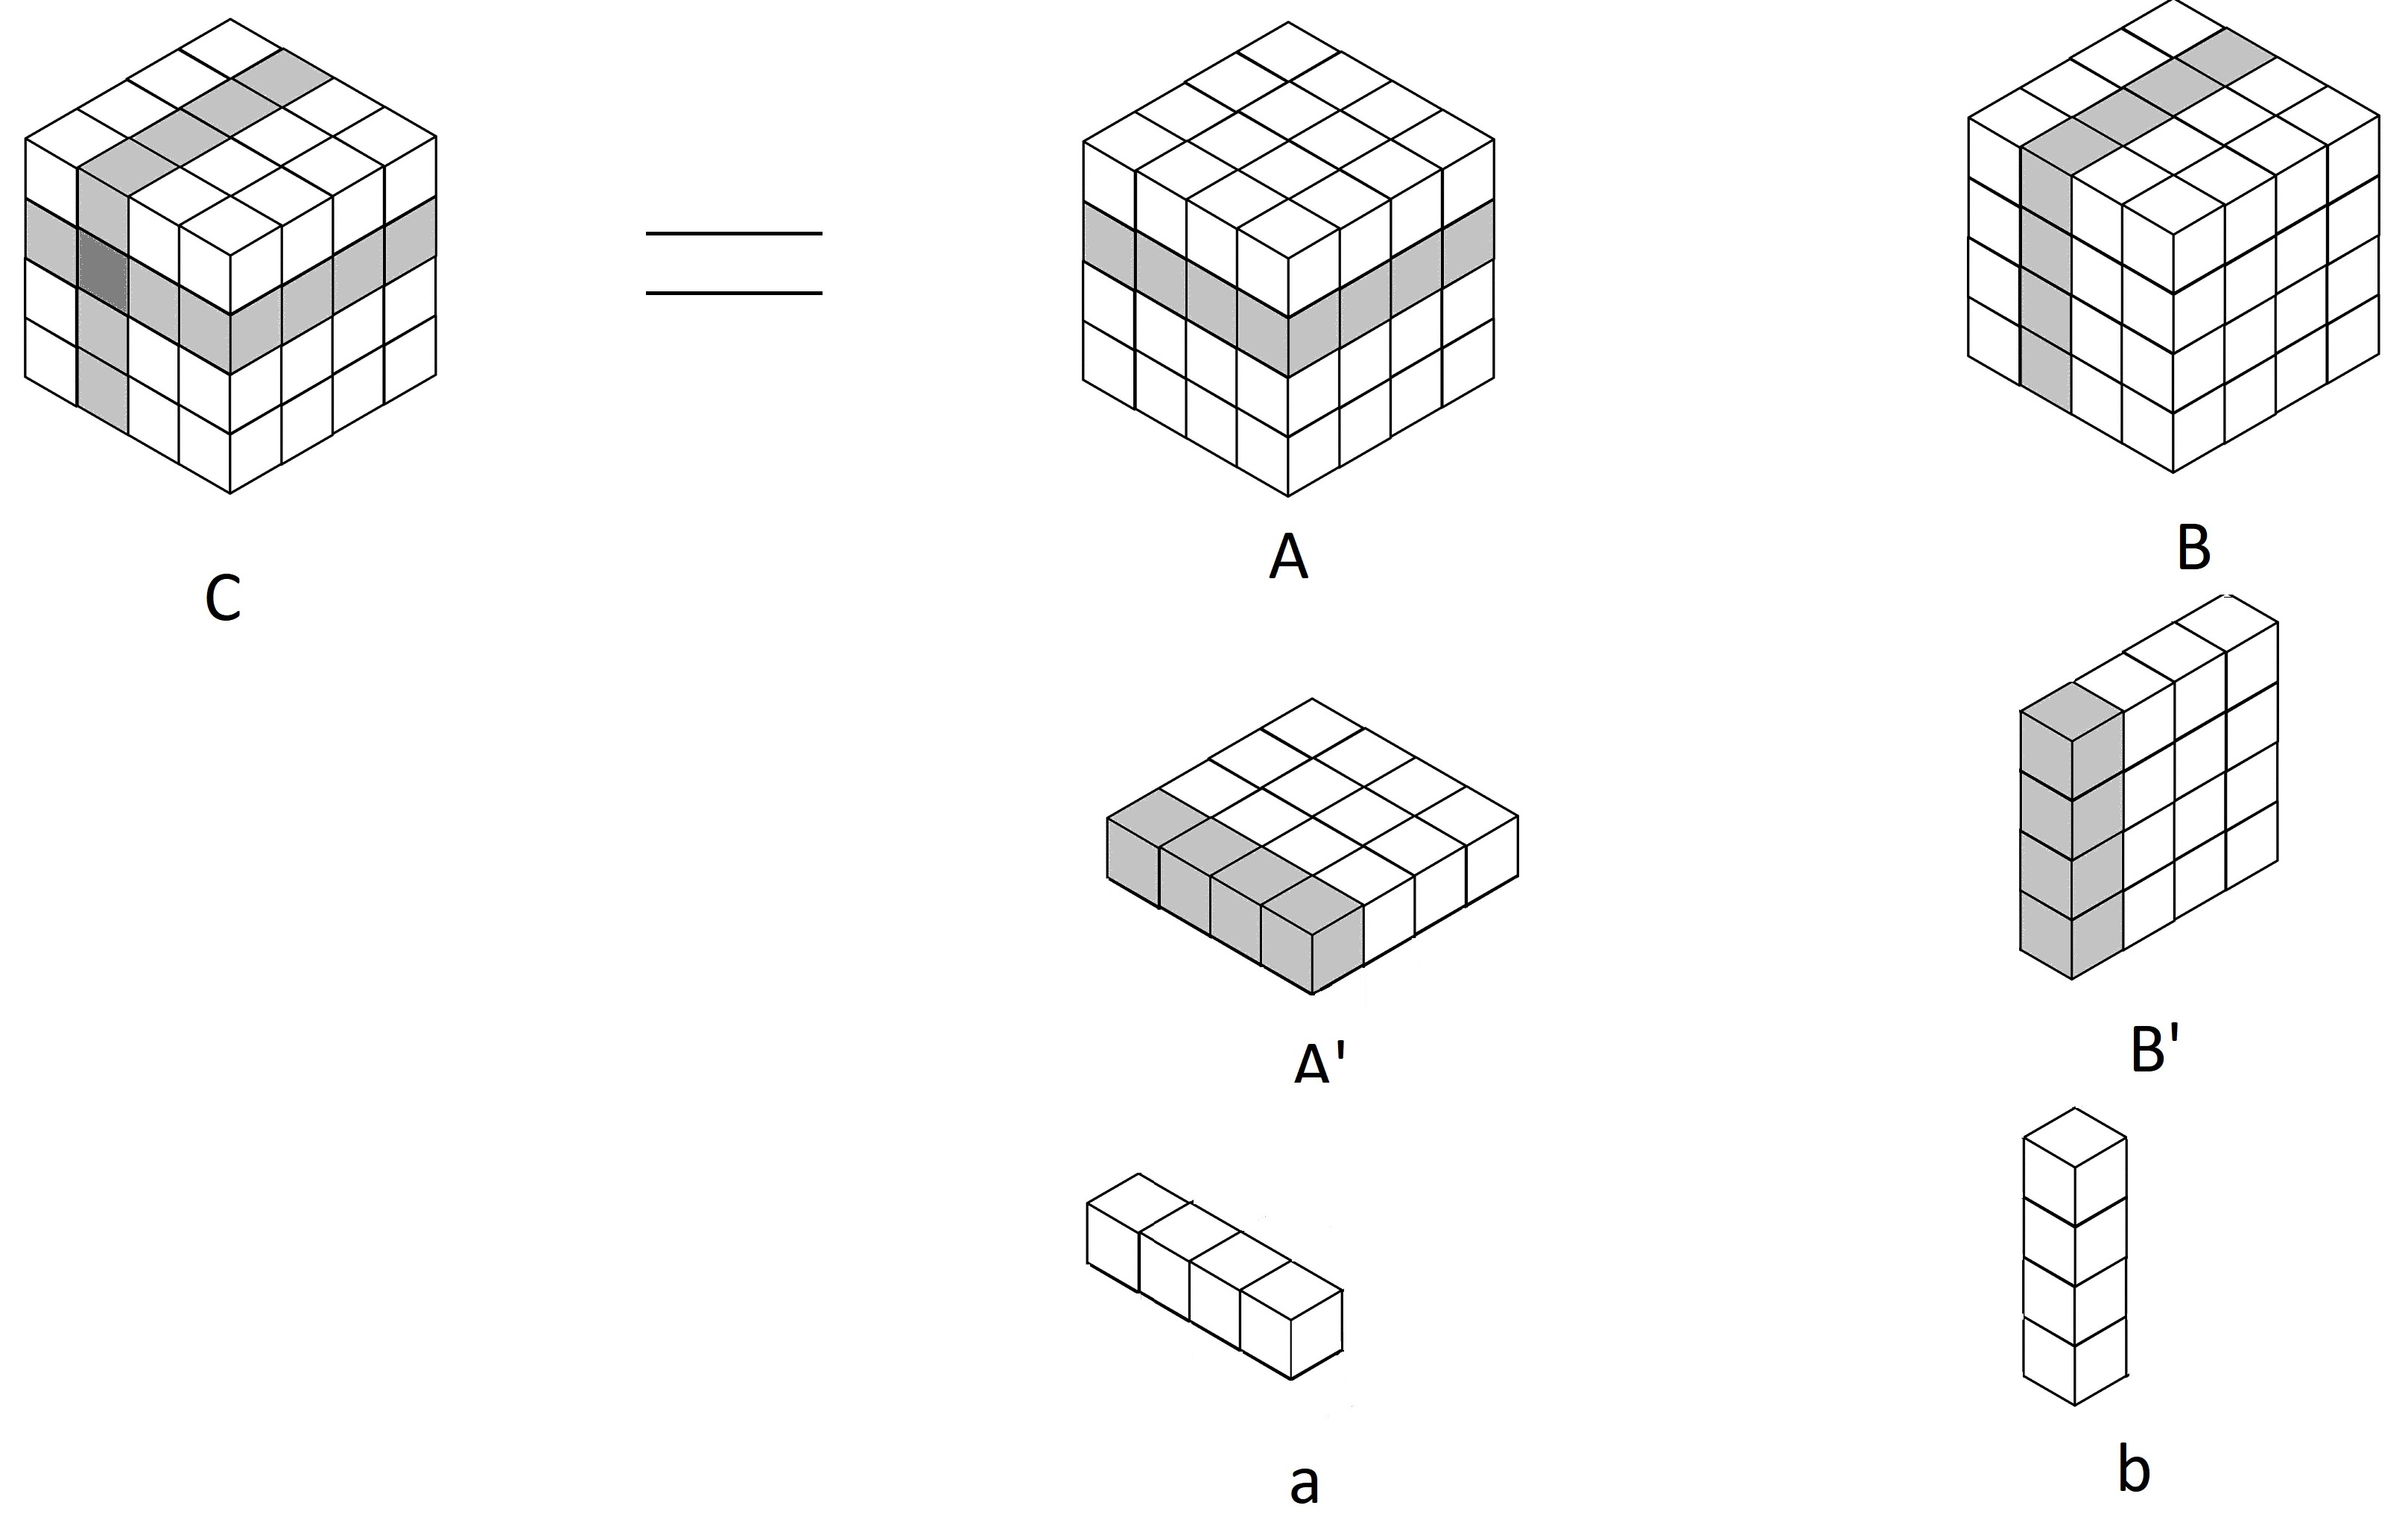
\includegraphics[scale=0.15]{3D.jpg}
\caption{CAPTION}\label{fig1}
\end{figure}

\begin{algorithm}[H]
\SetAlgoLined
\KwData{this text}
\KwResult{how to write algorithm with \LaTeX2e }
initialization\;
\While{not at end of this document}{
read current\;
\eIf{understand}{
go to next section\;
current section becomes this one\;
}{
go back to the beginning of current section\;
}
}
\caption{How to write algorithms}
\end{algorithm}

\end{document}